\documentclass{article}
\usepackage{graphicx}
\usepackage{float}
\usepackage{booktabs}
\usepackage{siunitx}
\usepackage{amsmath}


\title{Lab 6: Creating and Combining Sinusoids in MatLab}
\author{Sean Balbale}
\date{October 18th, 2024}
\setlength{\parindent}{0in}

\begin{document}

\begin{titlepage}
	\begin{center}
		\vspace*{1in}

		\Huge
		\textbf{Lab 6}

		\LARGE
		Creating and Combining Sinusoids in MatLab

		\vspace{3 in}

		\textbf{Student Name:} Sean Balbale
		\\ \textbf{Instructor:} Dr. Iman Salama
		\\ \textbf{Lab Partner Name:} Krish Gupta
		\\ \textbf{Date:} October 18, 2024

		\vfill


	\end{center}
\end{titlepage}

\newpage

\section{Introduction}
This lab focuses on the generation, analysis, and combination of discrete-time sinusoidal signals using MATLAB. 
Sinusoids, particularly sine and cosine waves, are fundamental to signal processing and electrical engineering applications, 
including biomedical signal analysis. The objective of this lab is to explore how varying parameters—amplitude, frequency, 
and phase—affect the behavior of sinusoidal signals in both visual and auditory contexts.

By generating, plotting, and combining sinusoids, we will observe the impact of these parameters on the shape, 
frequency content, and sound of the resulting signals. This hands-on approach deepens understanding of sinusoidal 
functions, which are integral to the study of circuits and signals, and prepares us for more complex applications in 
biomedical engineering and signal processing. MATLAB provides an efficient platform for simulating these signals and 
analyzing their properties, ensuring that we can accurately manipulate and study discrete-time signals.

\section{Results}
\subsection*{Part I}
\subsubsection*{A.}
\begin{figure}[H]
	\centering
	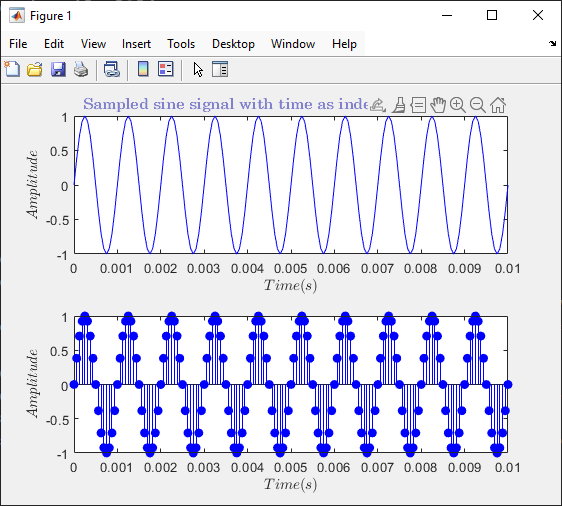
\includegraphics[width=0.5\textwidth]{fig 1a.png}
	\caption{Sinusoidal with $A$ = 1, $f$ 1 kHz, $f_s$ = 16 kHz, duration = 0.01, and Phase 0}
	\label{fig:fig1}
\end{figure}
In Figure \ref{fig:fig1}, we observe a sinusoidal signal with an amplitude ($A$) of 1, 
frequency ($f$) of 1 kHz, sampling frequency ($f_s$) of 16 kHz, duration of 0.01, 
and phase of 0. This results in 16 samples per cycle. This can be calculated through 
the formula:
\[ 
F = \frac{f}{f_s} = \frac{1000}{16000} = \frac{1}{16}
\]

\subsubsection*{B.}

\begin{figure}[H]
	\centering
	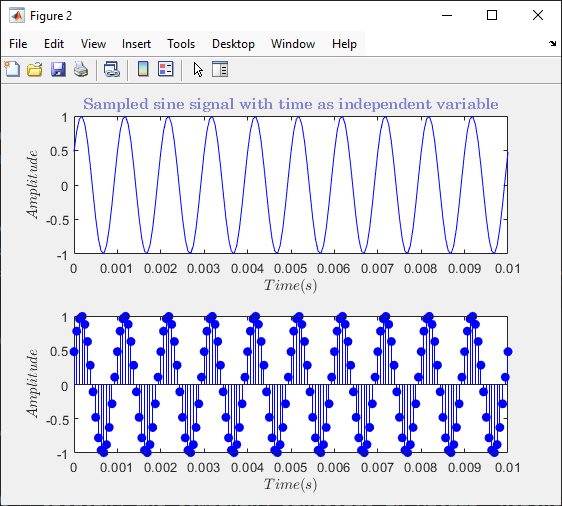
\includegraphics[width=0.5\textwidth]{fig 1b.png}
	\caption{Sinusoidal with $A$ = 1, $f$ 1 kHz, $f_s$ = 16 kHz, duration = 0.01, and Phase 0.5}
	\label{fig:fig2}
\end{figure}
As seen in Figure \ref{fig:fig2}, the sinusoidal signal has the same parameters as 
in part A, with the exception of the phase, which is now 0.5. This phase shift can be 
seen in the plot, where the signal starts at a different point in the cycle compared
to Figure \ref{fig:fig1}. The F value remains the same as in part A and there 
are still 16 samples per cycle.

\subsubsection*{C and D.}
For parts C and D, the sinusoidal signals have the same parameters as in parts A and B,
but with a duration of 1 second. The plots aren't useful for visualizing the signals,
but you can hear a beep that lasts one second. The phase shift between parts C and D
is not audible.


\subsubsection*{E.}
This part is the same as part D, but with an amplitude of 0.1. The amplitude of the
signal is reduced, resulting in a quieter beep. The phase shift is not audible.

\subsubsection*{F.}
For this part, part A is repeated but with sampling frequencies of 7000, 3000, and 
1300 Hz. 
\begin{figure}[H]
	\centering
	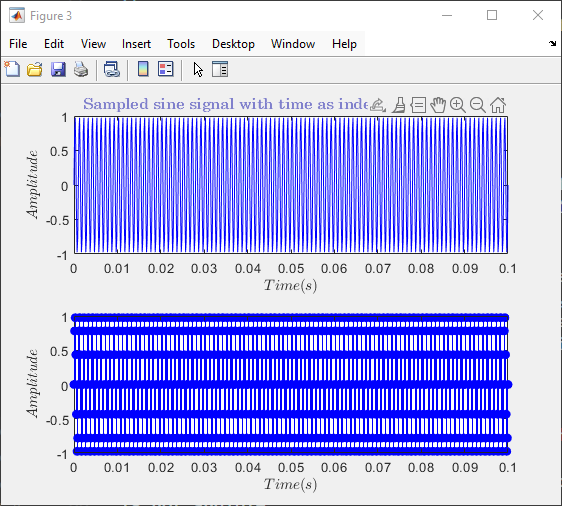
\includegraphics[width=0.3\textwidth]{fig 1f 7000.png}\hfill
	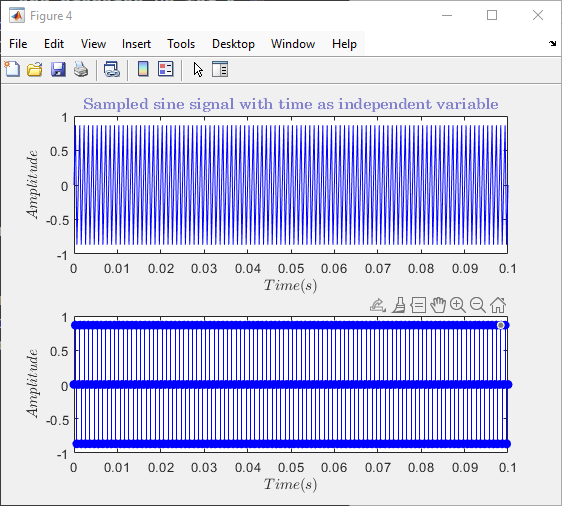
\includegraphics[width=0.3\textwidth]{fig 1f 3000.png}\hfill
	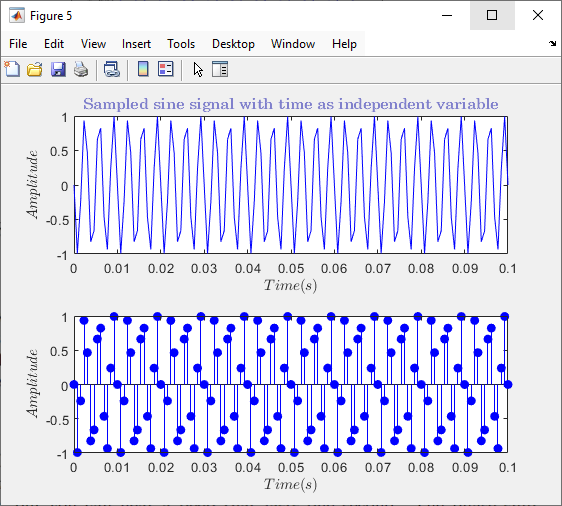
\includegraphics[width=0.3\textwidth]{fig 1f 1300.png}
	\caption{Sinusoidal with $f_s$ = 7 kHz, 3 kHz, and 1.3 kHz}
	\label{fig:fig3}
\end{figure}

As seen in Figure \ref{fig:fig3}, the sampling frequency affects the number of samples
per cycle. The signal with a sampling frequency of 7000 Hz has 7 samples per cycle, 
the signal with a sampling frequency of 3000 Hz has 3 samples per cycle, and the signal
with a sampling frequency of 1300 Hz has 1.3 samples per cycle. 

\subsubsection*{G.}
Here, part C is repeated with a sampling frequency of 7000 Hz, 3000 Hz, 1700 Hz, 
1300 Hz, and 1100 Hz. The sound of the beep decreases in quality and volume as the 
sampling frequency decreases. This is because the amount of sound data produced decreases.

\subsection*{Part II}
\subsubsection*{A.}
In this part, three sinusoidal signals are generated with frequencies of 1 kHz and 
amplitude values of 0.1, 0.3, and 1. The signals are then combined and plotted. In 
\ref{fig:fig4}, the three signals are shown. The signal with an amplitude of 0.1 is green,
the signal with an amplitude of 0.3 is blue, and the signal with an amplitude of 1 is red.
\begin{figure}[H]
	\centering
	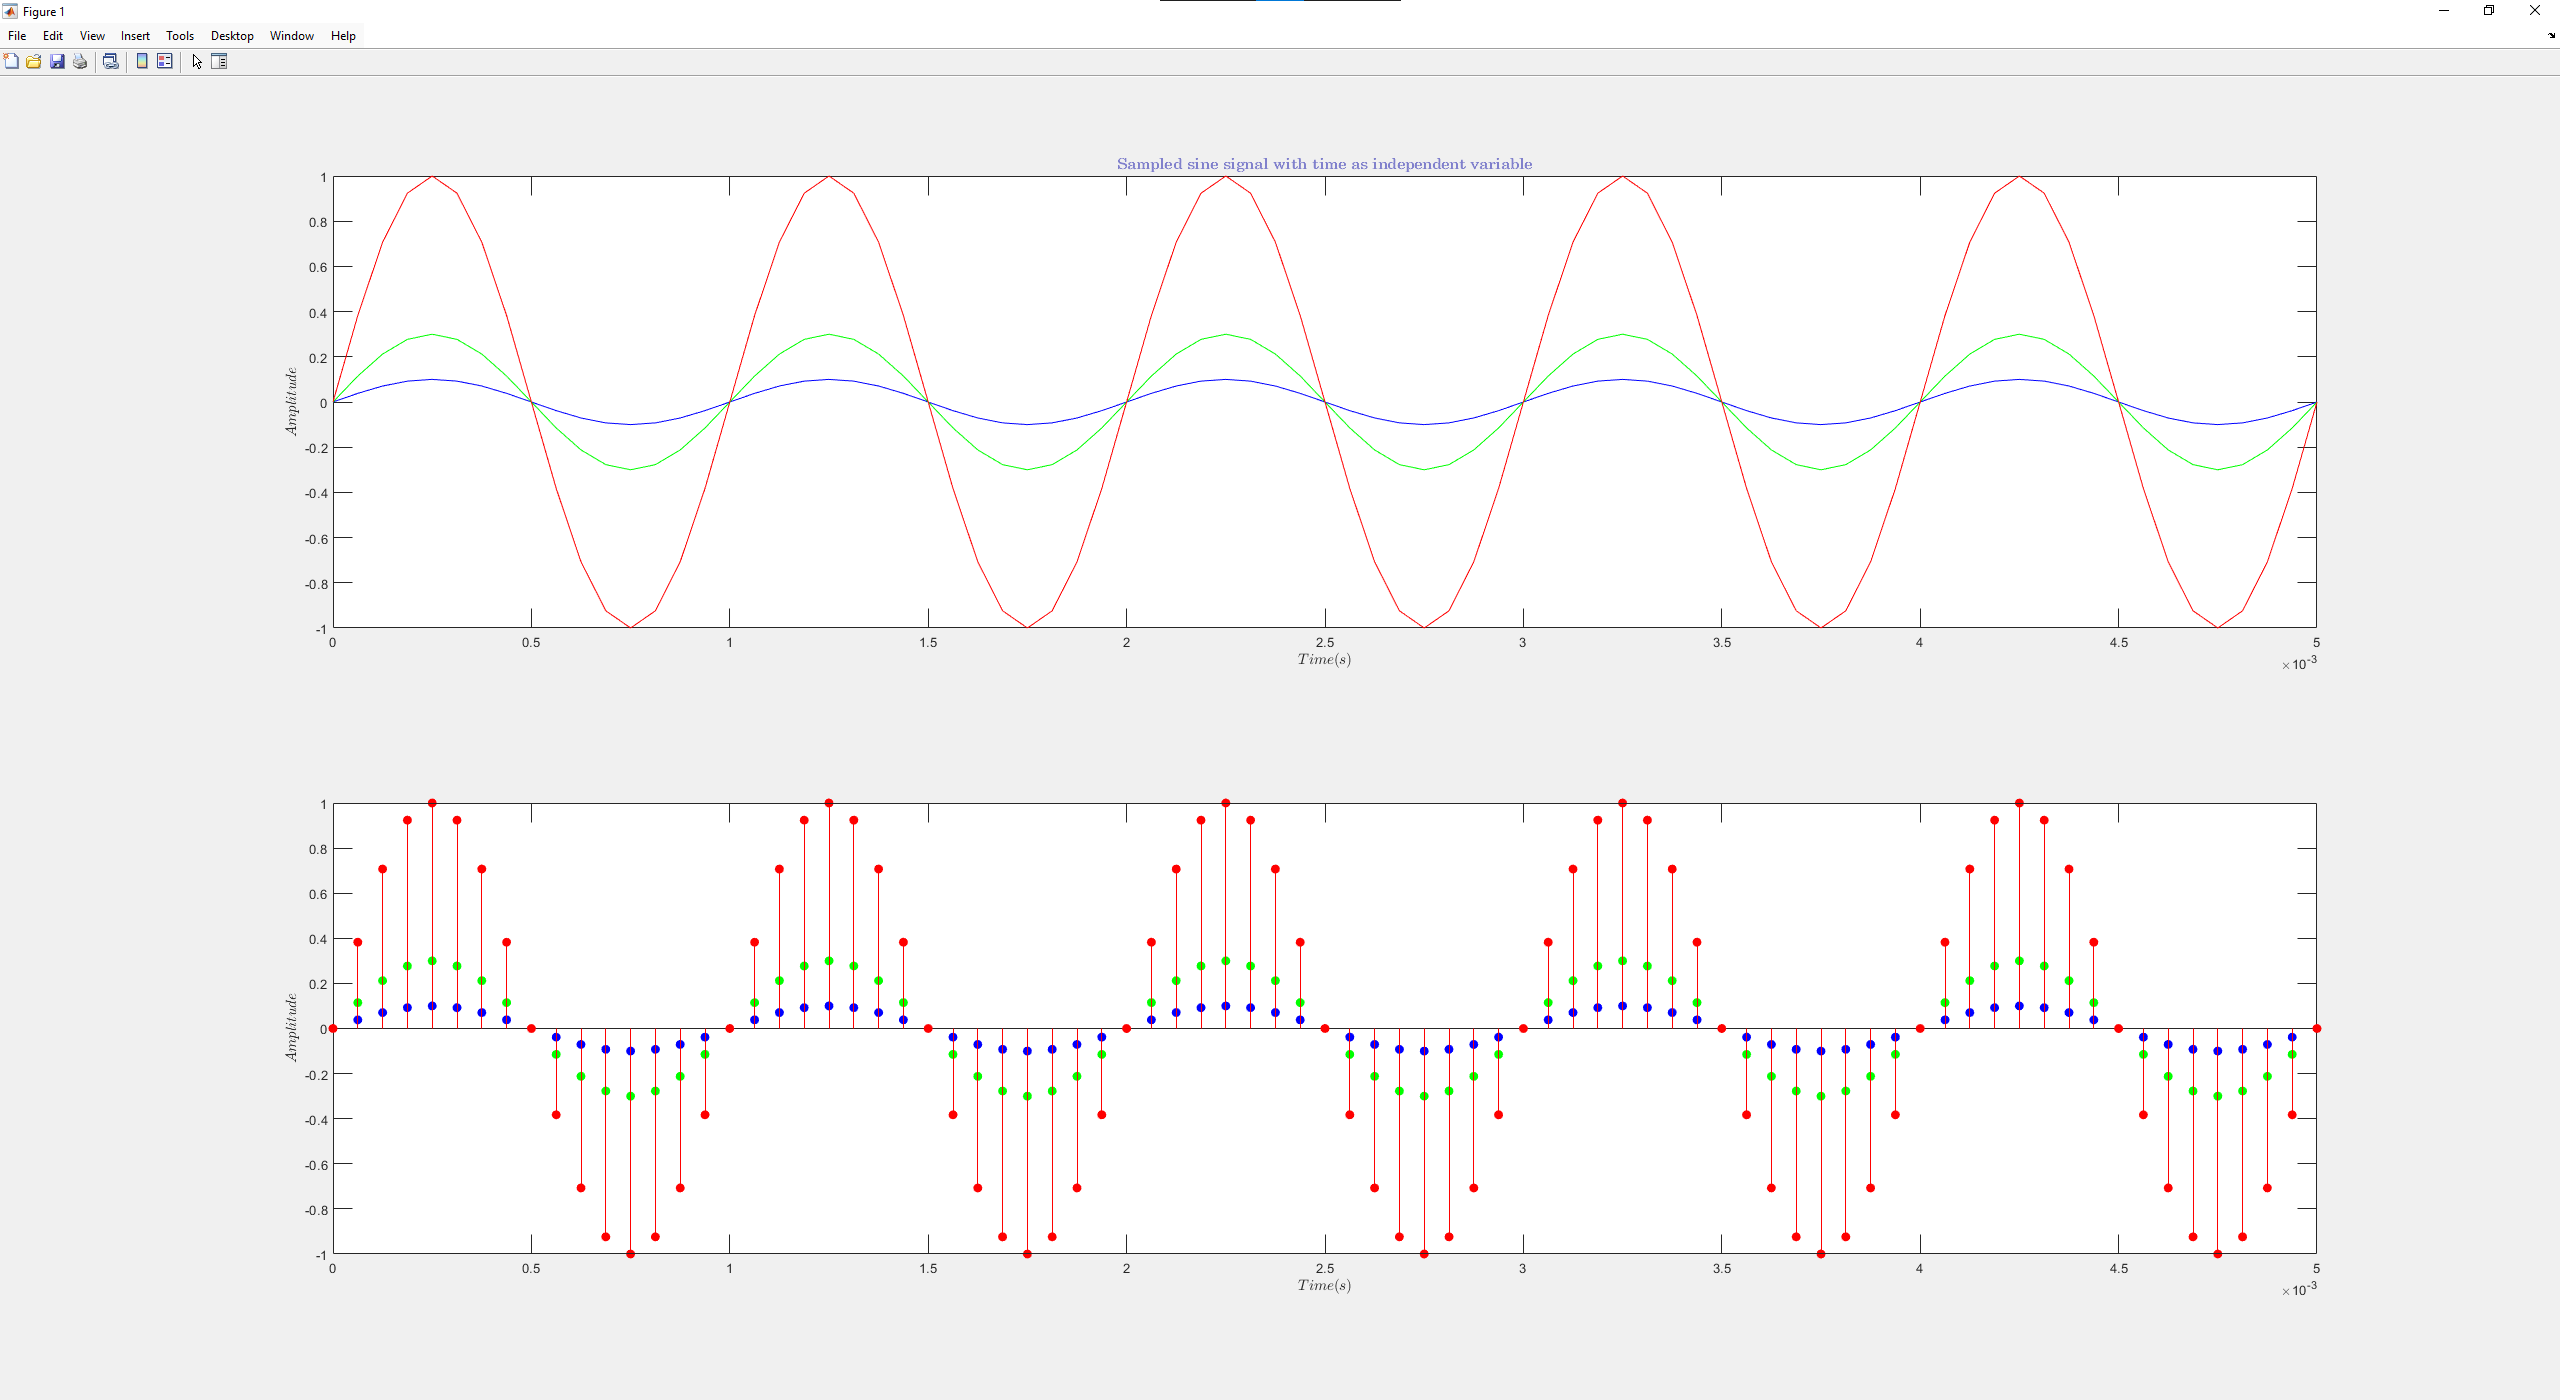
\includegraphics[width=0.75\textwidth]{fig 2a.png}
	\caption{Sinusoidal with $A$ = 0.1, 0.3, and 1}
	\label{fig:fig4}
\end{figure}

\subsubsection*{B.}
\begin{figure}[H]
	\centering
	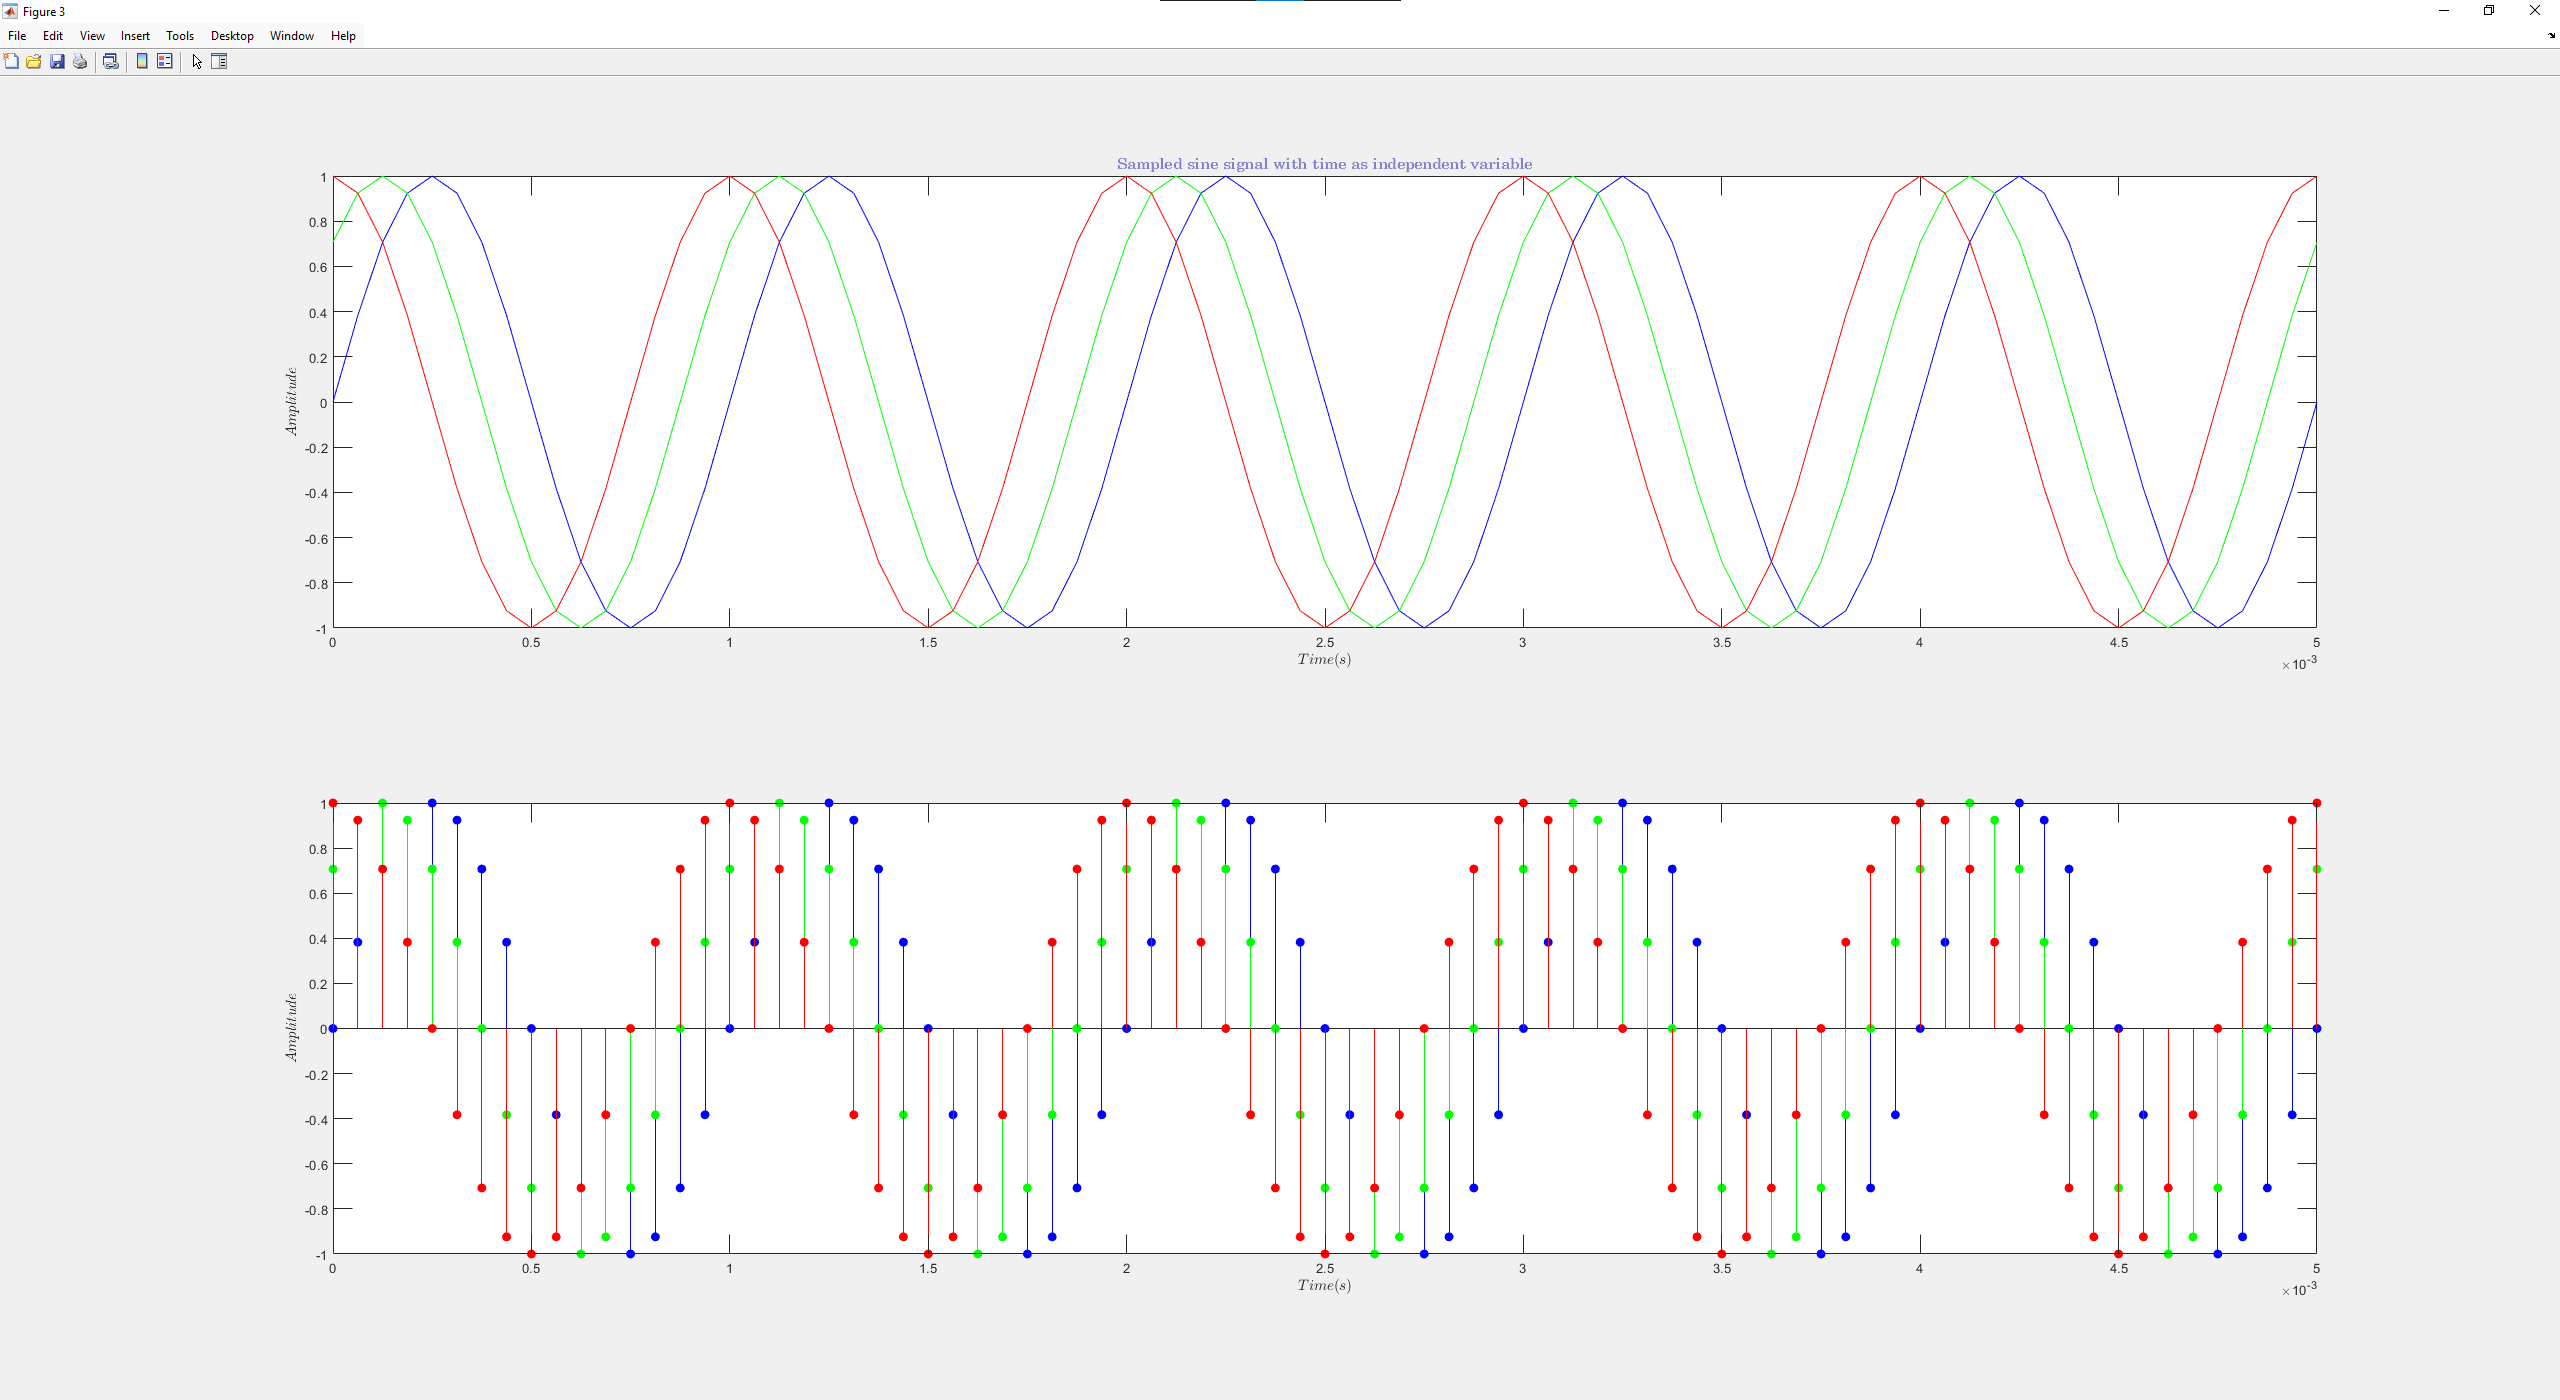
\includegraphics[width=0.5\textwidth]{fig 2b1.png}
	\caption{Sinusoidal with phase $\theta$ = 0,$\pi/4$, and $\pi/2$}
	\label{fig:fig5}
\end{figure}
In this part, three sinusoidal signals are generated with phase shifts of 0, $\pi/4$,
and $\pi/2$. The signals are then combined and plotted. In \ref{fig:fig5}. This is then
repeated with phase shifts of 0, $\pi$, and $4\pi$. The signals are then combined and 
plotted. In \ref{fig:fig6}, the signals are shown. 

\begin{figure}[H]
	\centering
	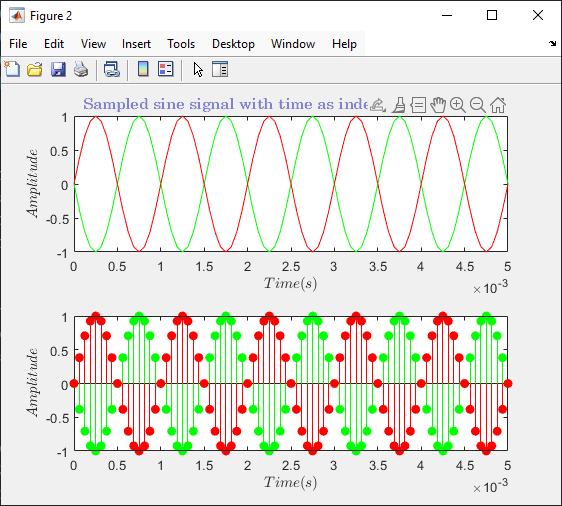
\includegraphics[width=0.5\textwidth]{fig 2b2.png}
	\caption{Sinusoidal with phase $\theta$ = 0,$\pi$, and $4\pi$}
	\label{fig:fig6}
\end{figure}

\subsubsection*{C.}
Part B is repeated but with 8000 samples instead of 250. Just like the results in Part I,
the phase shift is not audible.

\subsection*{Part III}
\subsubsection*{A.}

\section{Discussion and Conclusion}

\section{References}
 [1] Dr. Iman Salama. “Lab 6 – Creating and Combining Sinusoids in MatLab” Northeastern University. 18 October 2024.

\end{document}
